\documentclass[a4paper]{article}
\usepackage[utf8]{inputenc}
\usepackage[spanish, es-tabla]{babel}

\usepackage{amsmath}
\usepackage{amsfonts}
\usepackage{amssymb}

\usepackage{float}
\usepackage{graphicx}
\graphicspath{ {./Imagenes/} }

\usepackage{multirow}
\setlength{\doublerulesep}{\arrayrulewidth}

\usepackage{array}
\newcolumntype{C}[1]{>{\centering\let\newline\\\arraybackslash\hspace{0pt}}m{#1}}

\usepackage[american]{circuitikz}

\usepackage{fancyhdr}

\usepackage{units} 

\pagestyle{fancy}
\fancyhf{}
\lhead{22.02 Electrotecnia I}
\rhead{Mechoulam, Mestanza, Lambertucci, Pouthier, Londero}
\rfoot{Página \thepage}



\begin{document}

%%%%%%%%%%%%%%%%%%%%%%%%%%%%%%%%%%%%%%%%%%%%%%%%%%%%%%%%%%%%%%%%%%%%%%%%% 
%								CARATULA								%
%%%%%%%%%%%%%%%%%%%%%%%%%%%%%%%%%%%%%%%%%%%%%%%%%%%%%%%%%%%%%%%%%%%%%%%%% 

\begin{titlepage}
\newcommand{\HRule}{\rule{\linewidth}{0.5mm}}
\center
\mbox{\textsc{\LARGE \bfseries {Instituto Tecnológico de Buenos Aires}}}\\[1.5cm]
\textsc{\Large 22.02 Electrotecnia I}\\[0.5cm]


\HRule \\[0.6cm]
{ \Huge \bfseries Trabajo práctico N$^{\circ}$3}\\[0.4cm] 
\HRule \\[1.5cm]


{\large

\emph{Grupo 5}\\
\vspace{3px}

\begin{tabular}{lr} 	
\textsc{Mechoulam}, Alan  &  58438\\
\textsc{Lambertucci}, Guido Enrique  & 58009 \\
\textsc{Pouthier}, Florian  & 61337 \\
\textsc{Mestanza}, Nicolás  & 57521 \\
\textsc{Londero Bonaparte}, Tomás Guillermo  & 58150 \\
\end{tabular}

\vspace{20px}

\emph{Profesores}\\
\vspace{3px}
\textsc{Muñoz}, Claudio Marcelo\\ 	
\textsc{Ayub}, Gustavo\\ 	

\vspace{100px}

\begin{tabular}{ll}

Presentado: & 17/05/19\\

\end{tabular}

}

\vfill

\end{titlepage}


%%%%%%%%%%%%%%%%%%%%%%%%%%%%%%%%%%%%%%%%%%%%%%%%%%%%%%%%%%%%%%%%%%%%%%%%% 
%								INFORME									%
%%%%%%%%%%%%%%%%%%%%%%%%%%%%%%%%%%%%%%%%%%%%%%%%%%%%%%%%%%%%%%%%%%%%%%%%%

\section*{Introducción}

\section*{Desarrollo}

\subsection*{Simulación en LTSpice}

Se comenzó analizando el período de carga y descarga de los componentes capacitivos e inductivos del circuito dado.

\begin{figure}[H]
\begin{center}
\begin{circuitikz}
\draw
	(0,3) to [V,v_=$V$] (0,0)
	(0,0) to (4,0)
	(2,0) to [R, l_=$18 \ \Omega$] (2,1.5)
	(4,0) to [R, l_=$12 \ \Omega$] (4,1.5)
	(2,1.5) to [C, l_=$22 \ \mu f$]	(2,3)
	(4,3)	to [L, l=$13 \ mH$] (4,1.5)
	(0,3)	to [spst] (2,3)
	(2,3)	to (4,3)
	
;\end{circuitikz}
\caption{Circuito analizado.}
\end{center}
\end{figure}

Mediante el uso del programa \textbf{LTSpice}, y otorgando un valor arbitrario de $5 \ V$ a la tensión de entrada, se obtuvo

\begin{figure}[H]
	\centering
	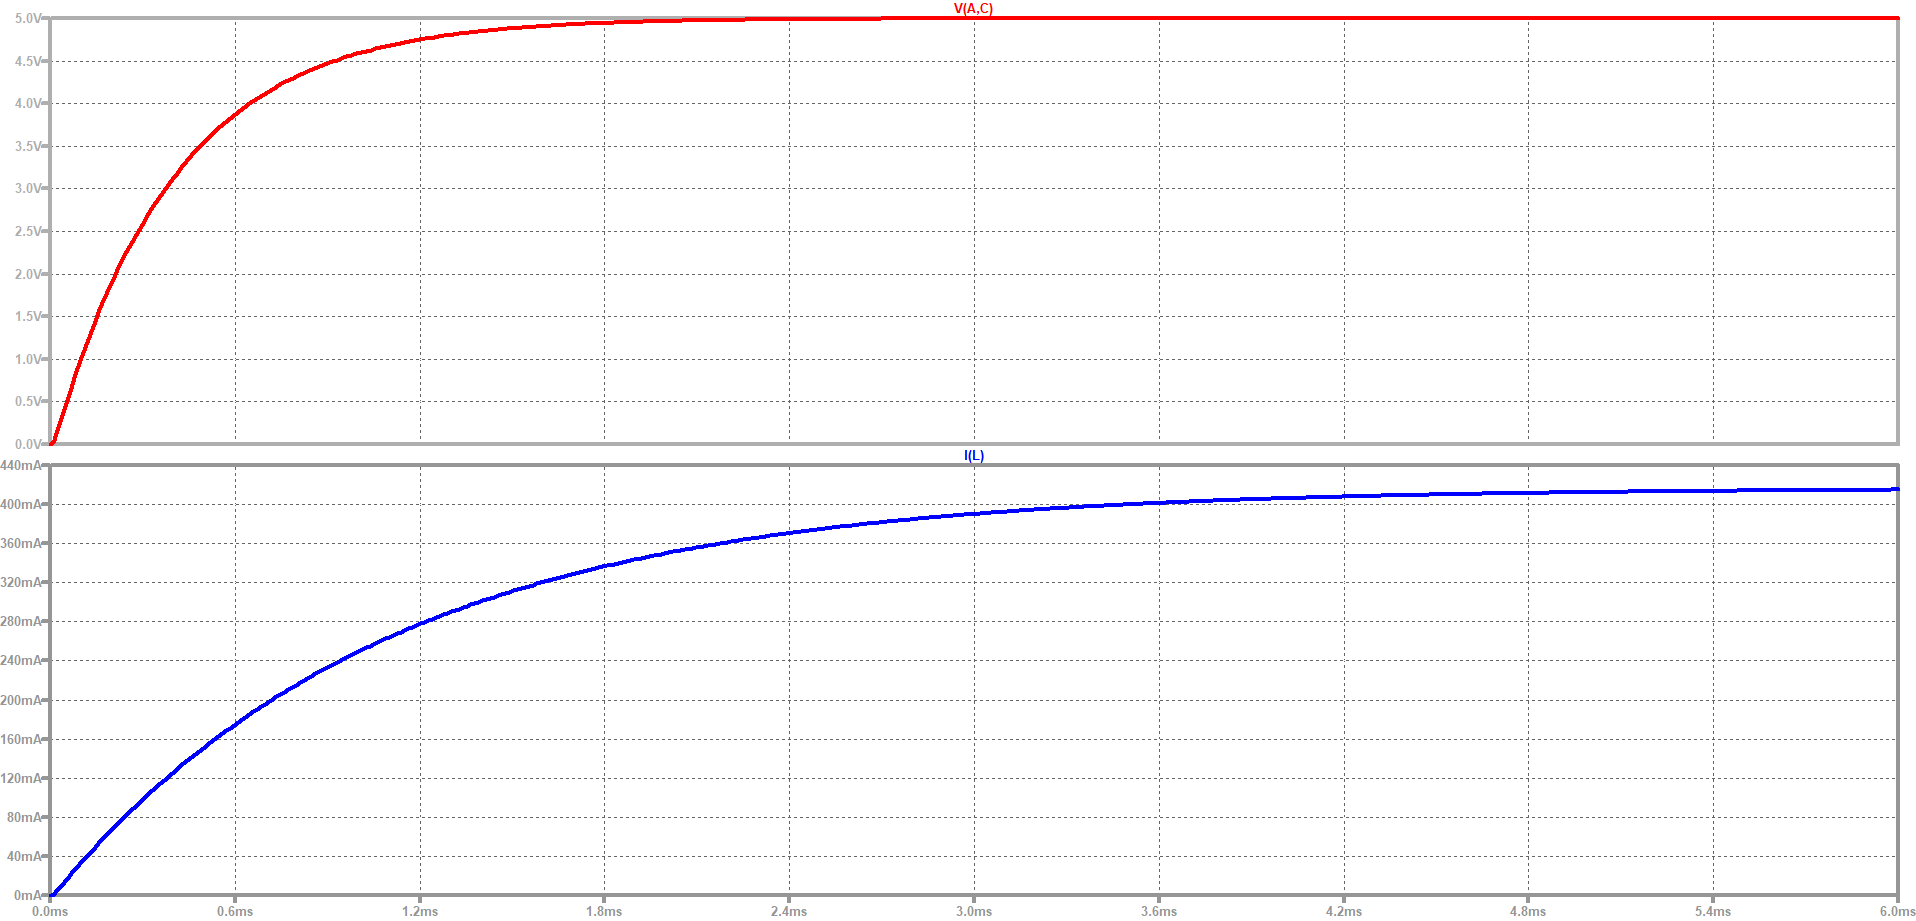
\includegraphics[width=\textwidth]{LTSpice-Carga1}
	\caption{Tensión del capacitor (en rojo) y corritente en la bobina (en azul) durante la carga.}
	\label{fig:LTSC1}
\end{figure}

\begin{figure}[H]
	\centering
	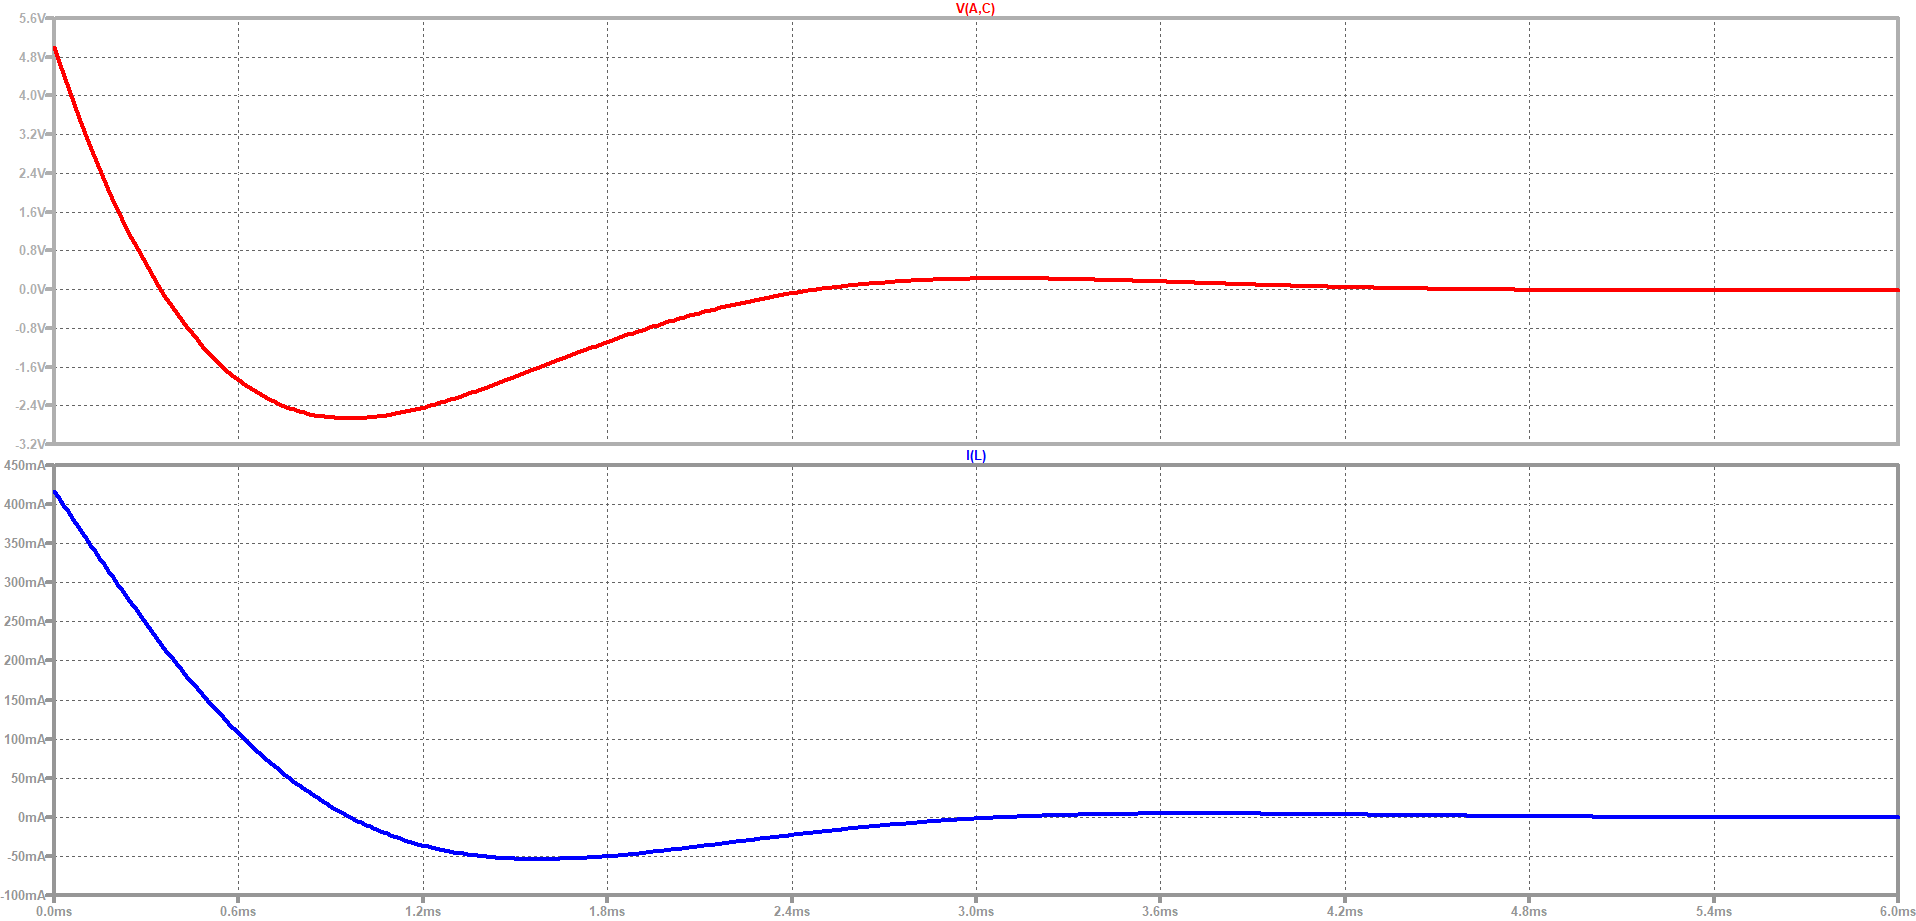
\includegraphics[width=\textwidth]{LTSpice-Descarga1}
	\caption{Tensión del capacitor (en rojo) y corritente en la bobina (en azul) durante la descarga.}
	\label{fig:LTSD1}
\end{figure}

Mediante el uso de las figuras (\ref{fig:LTSC1}) y (\ref{fig:LTSD1}) se pudo determinar la pseudofrecuencia de oscilación del transitorio y el valor máximo de sobrepico. De esta forma, se determinó para el capacitor una pseudofrecuencia de ${\omega}_{T} \ = \ 4.47 \ ms$ y un sobrepico de $227 \ mV$, y para el inductor una pseudofrecuencia de ${\omega}_{T} \ = \ 3.84 \ ms$ y un sobrepico de $4.55 \ mA$.

Para analizar teóricamente ambas situaciones se observa que tanto el capacitor como el inductor se encuentran en ramas distintas conectadas a una fuente de tensión constante, es por ello que se llega a las siguientes ecuaciones:

\begin{equation}
	V_{C} (t) = V_{f} \left( 1 - e^{- \frac{t}{0.396 \ ms}  } \right)
	\label{eq:carg-c}
\end{equation}

\begin{equation}
	I_{L} (t) = V_{f} \left( 1 - e^{- \frac{t}{0.156 \ s}  } \right)
	\label{eq:carg-l}
\end{equation}

Por otro lado, para la descarga, el circuito es un RLC serie. Sabiendo que para este circuito $\alpha < \omega_0$, se plantea la solución para un circuito subamortiguado, obteniéndose así las siguientes ecuaciones:

\begin{equation}
	V_{C} (t) = V_{f} \cdot e^{- \alpha t} \left[ cos \left(  \omega_d t \right) + {\omega_d}^{-1}  \left( \alpha + \frac{R}{C} \right) sen \left(  \omega_d t \right) \right]
	\label{eq:descarg-c}
\end{equation}

\begin{equation} \label{eq:descarg-l}
\begin{split}
I_{L} (t) = V_{f} C \cdot e^{- \alpha t} \left\lbrace - \alpha \left[ cos \left(  \omega_d t \right) + {\omega_d}^{-1}  \left( \alpha + \frac{R}{C} \right) sen \left(  \omega_d t \right) \right] \right. \\
 \left. - \omega_d sen \left(  \omega_d t \right) + \left( \alpha + \frac{R}{C} \right) cos \left(  \omega_d t \right) \right\rbrace
\end{split}
\end{equation}

con $\alpha = 1153.85 \ \frac{1}{s}$, $\omega_d = 1471.44 \ \frac{1}{s}$, $R = 30 \ \Omega$.

Luego se analiza el caso en el cual el valor de ambas resistencias sea de $0 \ \Omega$. Dicha situación no es posible en la realidad ya que siempre se presenta una resistencia interna por parte de los elementos. Idealmente, lo que sucedería sería que la tensión y la corriente oscilarían sin perdidas de energía.

Finalmente, se realizó un diagrama de Montecarlo. Para ello se determinó las tolerancias de los distintos componentes de la siguiente forma: 5\% para las resistencias, 10\% para el capacitor y 0\% para la bobina. Se corrió la simulación 100 veces con un punto inicial en 1 e incrementándolo en 1 por iteratición. Además, se configuró la fuente de tensión de entrada para que varíe desde $0 \ V$ a $5 \ V$ con un paso de $0,1 \ V$. De esta forma se obtuvieron los gráficos presentados en la figuras (\ref{fig:LTSMCVC}), (\ref{fig:LTSMCIL}) y (\ref{fig:LTSMCIR}).

\begin{figure}[H]
	\centering
	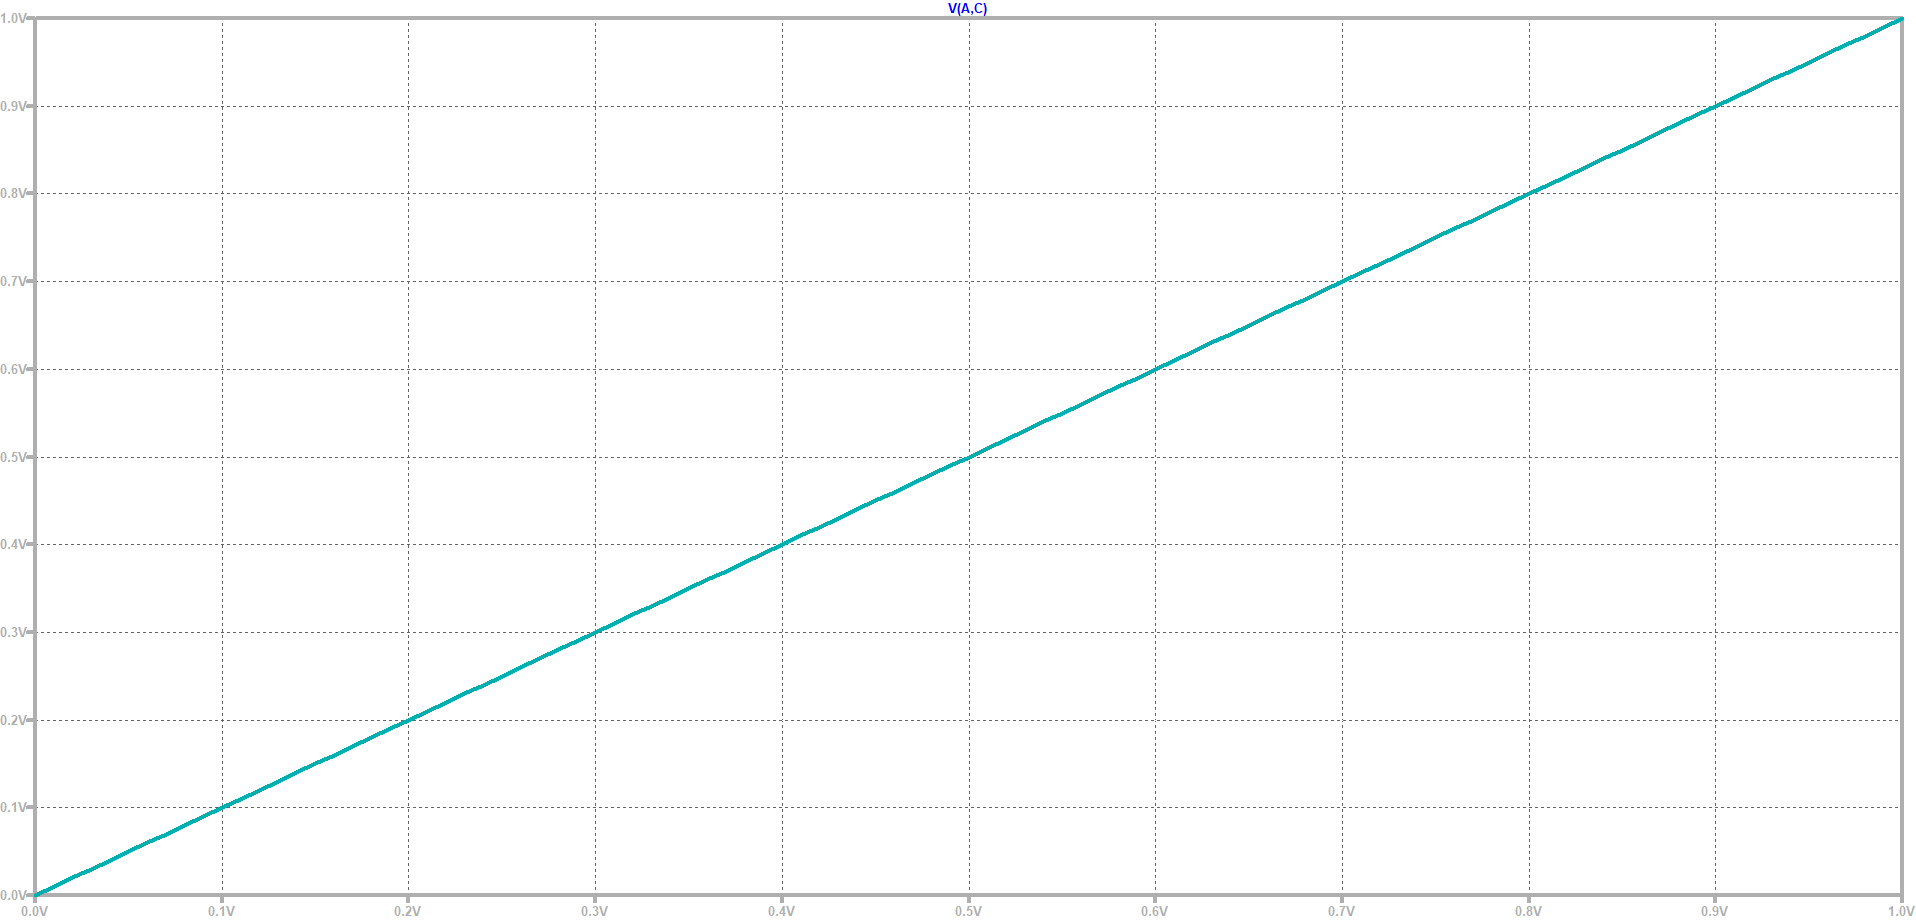
\includegraphics[width=\textwidth]{LTSpice-MC1-VC}
	\caption{Análisis de Montecarlo de la tensión en el capacitor.}
	\label{fig:LTSMCVC}
\end{figure}

\begin{figure}[H]
	\centering
	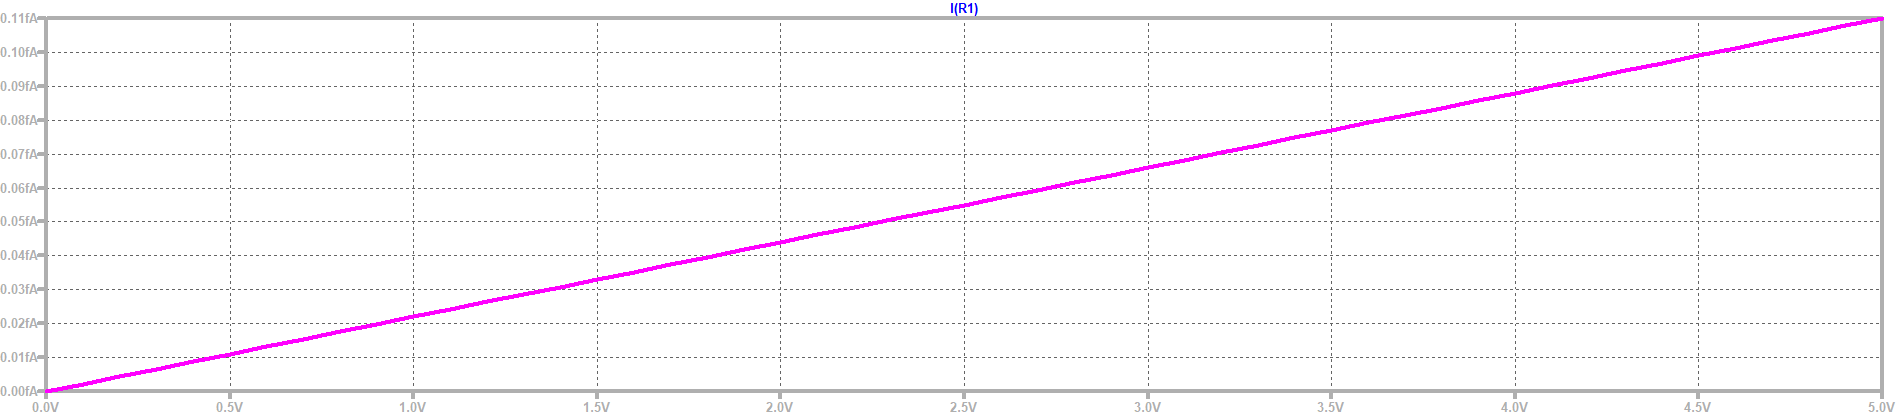
\includegraphics[width=\textwidth]{LTSpice-MC1-IR}
	\caption{Análisis de Montecarlo de la corriente en la resistencia 1.}
	\label{fig:LTSMCIR}
\end{figure}

\begin{figure}[H]
	\centering
	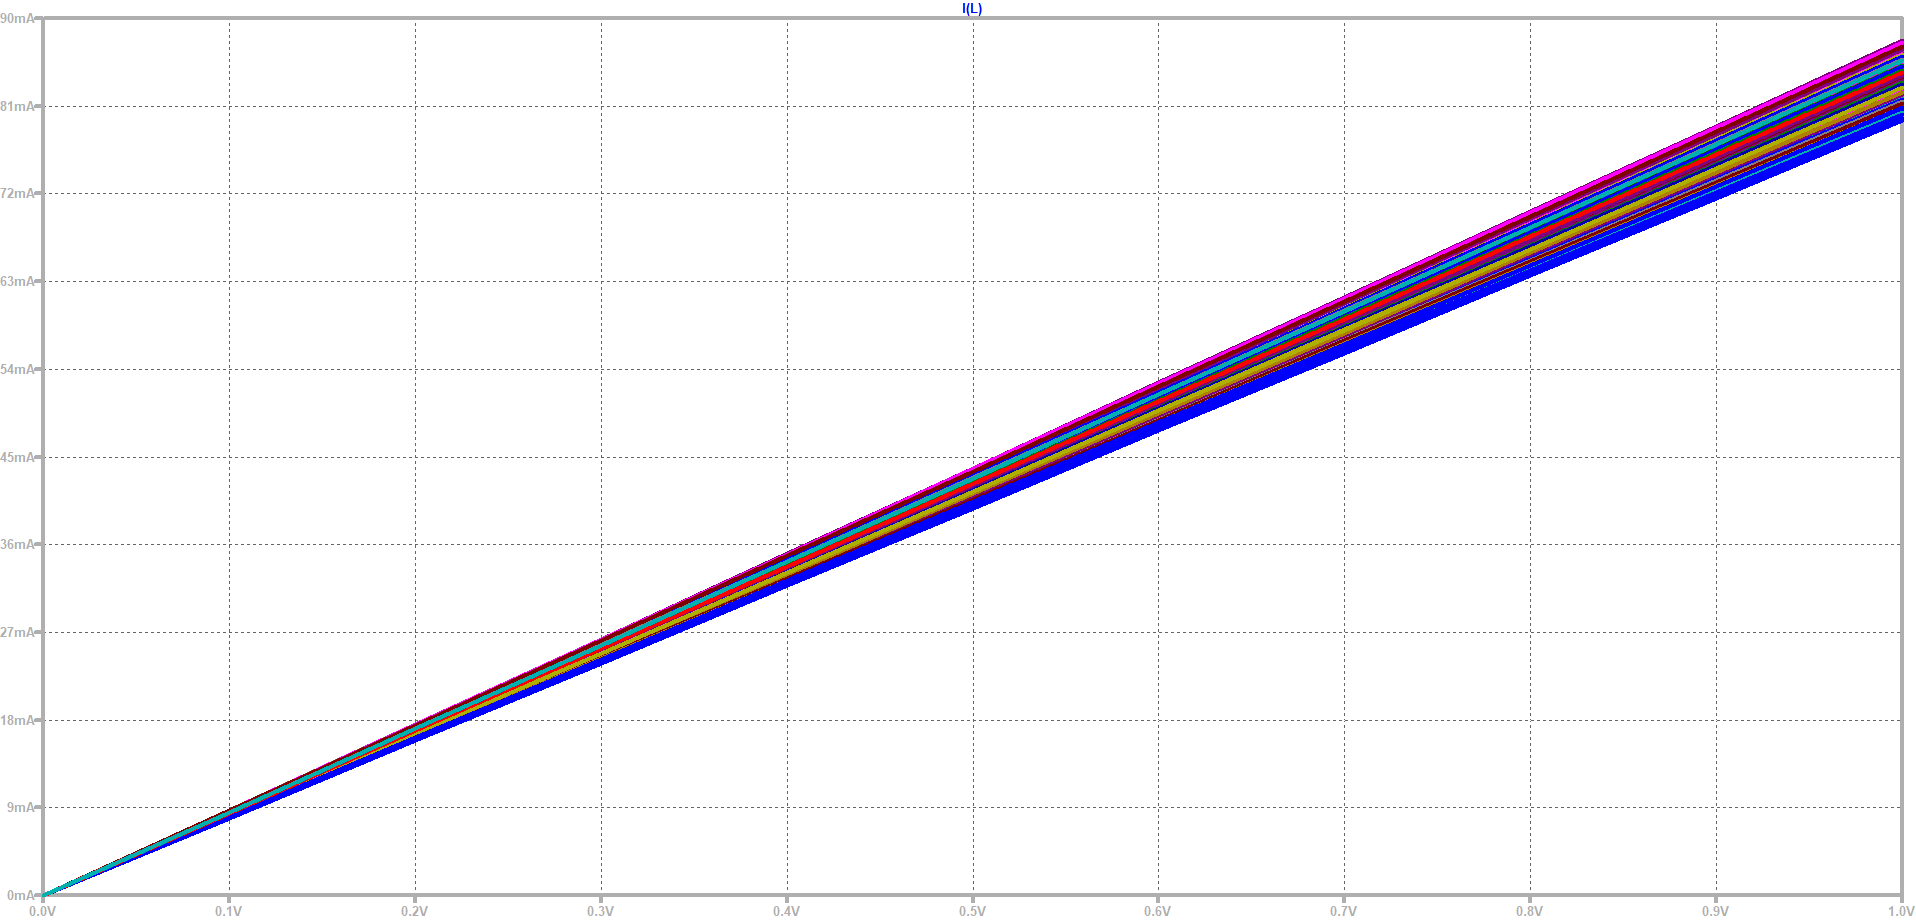
\includegraphics[width=\textwidth]{LTSpice-MC1-IL}
	\caption{Análisis de Montecarlo de la corriente en la bobina (igual corriente que en la resistencia 2).}
	\label{fig:LTSMCIL}
\end{figure}

\section*{Conclusión}


\end{document}
